\chapter{Algorithms}

In this section, we will go through several optimization algorithms and some bounds.

\section{Algorithm: Gradient Descent}
One of the most famous and frequently used optimization algorithms is the gradient descent, which can be formulated as:
\begin{equation}\label{eq:GradientDescentUpdateFormula}
    x_{k+1} \leftarrow x_k - \alpha_k\nabla f(x_k)
\end{equation}
Interestingly, this update formula can be interpreted in the following way:
\begin{equation*}
    x_{k+1} = \argmin_x \{ f(x_k) + \langle \nabla f(x_k), x-x_k \rangle + \frac{1}{2\alpha_k}\|x-x_k\|^2 \}
\end{equation*}
This means $x_{k+1}$ is the minimizer of the first-order approximation under quadratic distance penalty. In fact, if we denote $h(x) = f(x_k) + \langle \nabla f(x_k), x-x_k \rangle + \frac{1}{2\alpha_k}\|x-x_k\|^2$, by checking the first-order necessary condition, we have 
\begin{equation*}
    \nabla h(x) = \nabla f(x_k) + \frac{1}{\alpha_k}(x - x_k)
\end{equation*}
By setting $\nabla h(x) = 0$, we derive $x_{k+1} = x = x_k - \alpha_k\nabla f(x_k)$, which is the same as formula \ref{eq:GradientDescentUpdateFormula}.

\begin{note}
    One straightforward understanding of $\alpha_k$ is the step size taken as illustrated in \ref{eq:GradientDescentUpdateFormula}. However, as a quadratic in $h(x)$, it also represents how tolerant we are to distant condidates. Higher $\alpha_k$ indicates greater tolerance, corresponding to the gentler speed of change in the quadratic. 
\end{note}

Since we are interested in the minimization and maximization potential of the update algorithm, it's worth to explore how the corresponding value $f(x)$ changes. 
\begin{lemma}[Descent Lemma]\label{lemma:DescentLemma}
    Let $f: \mathbb{R}^d \rightarrow \mathbb{R}$ have L-Lipschitz gradient and $k \geq 0$, we have
    \begin{equation*}
        f(x_{k+1}) \leq f(x_k) - (\alpha_k - \frac{L\alpha_k^2}{2}) \| \nabla f(x_k) \|^2
    \end{equation*}
\end{lemma}
\begin{proof}
    Only need to use the first-order Taylor bound:
    \begin{equation*}
        | f(x_{k+1}) - f(x_k) - \langle \nabla f(x_k), x_{k+1} - x_k \rangle | \leq \frac{L}{2}\|x_{k+1} - x_k\|^2
    \end{equation*}
\end{proof}

\begin{corollary}
    If we take $\alpha_k = \frac{1}{L}$ as in exact linesearch, then we have:
    \begin{equation*}
        f(x_{k+1}) \leq f(x_k) - \frac{1}{2L} \| \nabla f(x_k) \|^2
    \end{equation*}
\end{corollary}

To minimize $f(x)$, we want the upper bound in lemma \ref{lemma:DescentLemma} to be as small as possible, meaning that we need to maximize $\alpha_k - \frac{L\alpha_k^2}{2}$. By solving this simple quadratic, we derive the ideal step size $\alpha_k = \frac{1}{L}$. However, this can be quite impractical since even if it's not a strong assumption to take functions we see in real life over a fintie domain as Lipschitz, it can be difficult to determine the Lipschitz constant $L$ for an unknown function. If we examine the update formula \ref{eq:GradientDescentUpdateFormula} closely, the only thing that needs external care is the step size $\alpha_k$. As a result, in the following we will discuss how to find a both effectively and pratically way to determine the step size $\alpha_k$.

\subsection{Exact Linesearch}

A straight forward approach is to find the solution of the following optimization problem, which is also referred to as the exact line search:
\begin{equation*}
    \alpha_k = \argmin_{\alpha \in \mathbb{R}}f(x_k - \alpha\nabla f(x_k))
\end{equation*}
Yet this can also be impractical because it means we have to solve an optimization problem at each step of update. In replacement to exact linesearch, we introduce the following backtracking linesearch algorithm by \emph{Larry Armijo}.

\subsection{Backtracking Linesearch}
The idea of backtracking linesearch is quite simple, we start with a step size large enough, and then shrink it little by little until we observe sufficient descent in $f(x)$. This can be formalized with the following two steps:
\begin{enumerate}
    \item Pick $\alpha \in \mathbb{R}_{>0}$ and $\tau \in (0,1)$, decrease step size by $\alpha_n = a\tau^n$.
    \item To measure the descent, we use the so-called Armijo condition.
\end{enumerate}
\begin{definition}[Armijo Condition]\label{def:ArmijoCondition}
    Pick $\eta \in (0,1)$, declare sufficient descent when 
    \begin{equation*}
        f(x_{k+1}) = f(x_k - \alpha\nabla f(x_k)) \leq f(x_k) - \eta\alpha\|\nabla f(x_k)\|^2
    \end{equation*}
\end{definition}

Therefore, we can restate the backtracking algorithm as:
\begin{equation*}
    \alpha_k = \max_n \{ a\tau^n : \text{Armijo condition holds for }\alpha = a\tau^n \}
\end{equation*}
One nice thing about Armijo's condition is that it clarifies the vague term "sufficient decsent". Beacuse we have $\eta \in (0,1)$, we certainly have the linear upper bound in \ref{def:ArmijoCondition} to be greater than $f(x - \alpha \cdot \nabla f(x))$ for $\alpha \in (0, \epsilon)$. One thing worth noticing is that, for $\eta$ small enough, it is possible for us to obtain multiple disconnected intervals with $\alpha$ satisfying the sufficient descent condition like $\eta = 0.3$.

\begin{figure}[H]
    \centering
    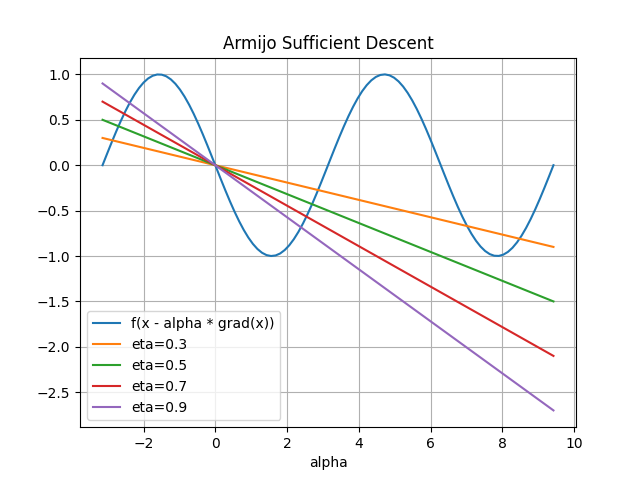
\includegraphics[scale=0.6]{plot_maker/Armijo_Sufficient_Descent/Armijo_sufficient_descent.png}
\end{figure}

Specifically, the following lemma describes the first Armijo interval near 0.

\begin{lemma}\label{lemma:ArmijoStepSizeBound}
    The Armijo condition holds for 
    \begin{equation*}
        \alpha \in [0, \frac{2(1 - \eta)}{L}]
    \end{equation*}
\end{lemma}
\begin{proof}
    Using the descent lemma, and bound the right hand side with linear upper bound, we have
    \begin{equation*}
        f(x_k - \alpha \nabla f(x_k)) \leq f(x_k) - (\alpha - \frac{L\alpha^2}{2})\|\nabla f(x_k)\|^2 \leq f(x_k) - \eta\alpha\|\nabla f(x_k) \|^2
    \end{equation*}
    This is the same as
    \begin{equation*}
        \eta\alpha \leq \alpha - \frac{L}{2}\alpha^2
    \end{equation*}
\end{proof}

\begin{note}[Consequences of Backtracking Linesearch]
    Firstly, in searching for step size $\alpha$, it needs no more than $\lceil \log_{\frac{1}{\tau}} (\frac{\alpha L}{2(1-\eta)}) \rceil $ steps to terminate. This bound is derived by asking $\alpha \tau^n \leq $ the bound in \ref{lemma:ArmijoStepSizeBound}. Secondly, we have $\alpha_k \geq \min\{ a, \frac{2\tau(1 - \eta)}{L} \}$ because we either find the sufficient descent at the first step, or find it no smaller than $\tau$ times the upper bound in \ref{lemma:ArmijoStepSizeBound}, which is the next iteration of step size. So we can rewrite the Armijo condition as:
    \begin{align}
        f(x_{k+1}) &\leq f(x_k) - \eta \alpha_k\|\nabla f(x_k) \|^2 \\
        &\leq f(x_k) - \eta \min\{ a, \frac{2\tau(1-\eta)}{L} \} \cdot \|\nabla f(x_k) \|^2  \label{eq:ArmijoUpdateBound}
    \end{align}
    Now in the special case where $a \geq \frac{1}{L}$ and $\eta = \tau = \frac{1}{2}$, we have 
    \begin{align*}
        (\ref{eq:ArmijoUpdateBound}) &\leq f(x_k) - \frac{1}{2}\min\{\frac{1}{L}, \frac{1}{2L}\} \cdot \|\nabla f(x_k) \|^2 \\
        &\leq f(x_k) - \frac{1}{4L}\| \nabla f(x_k) \|^2
    \end{align*}
    which does not result in a great sacrifice on the tightness of the bound compared with the quadratic in the descent lemma when the step size is small enough or asking $L > 1$. 
    
    A plot is available at \emph{Nonlinear\_Optimization/plot\_maker/Armijo\_and\_Descent\_Bound/plot.py}, python=3.11.5 + holoviews.
\end{note}

\section{NonConvex Smooth Optimization Guarantee}
Equipped with the bounding results on $f(x_{k+1})$ from the previous chapter, without convexity, we will see what we can say about L-smooth function and update rule:
\begin{equation*}
    x_{k+1} \leftarrow x_k - \alpha_k \nabla f(x_k)
\end{equation*}

\begin{theorem}[Bound on Average Gradient Norm for Nonconvex Functions]\label{thm:NonconvexGradientNormBound}
    Suppose $f(x)$ is L-smooth, then for any $T > 0$, we have:
    \begin{equation*}
        \frac{1}{T}\sum_{k=0}^{T-1}\|\nabla f(x_k) \|^2 \leq \frac{2L}{T}(f(x_0) - \min_{0\leq k \leq T-1}f(x_k)) \leq \frac{2L}{T}(f(x_0) - \min_{x \in \mathbb{R}^d}f(x)) 
    \end{equation*}
    when we set $\alpha_k = \frac{1}{L}$, i.e. exact linesearch.

    In addition, with Armijo backtracking, we have:
    \begin{equation*}
        \frac{1}{T}\sum_{k=0}^{T-1}\|\nabla f(x_k) \|^2 \leq \frac{\max \{ \frac{1}{\eta a}, \frac{L}{2\tau\eta(1-\eta)} \}}{T}(f(x_0) - \min_{x \in \mathbb{R}^d}f(x))
    \end{equation*}
\end{theorem}
\begin{proof}
    Use the bound of $f(x_{k+1})$ we derived from the previous section, i.e. descent lemma \ref{lemma:DescentLemma} and Armijo. Sum all of the inequalities up, then change $f(x_k)$ to $\min f(x)$
\end{proof}

This theorem describes the average pattern of the sequence of the gradients $\{ \nabla f(x_k) \}$, it indicates that there exists at least one $x_k^*$ such that $\| \nabla f(x_k^*) \|$ itself satisfies the inequality. Now let's first define what is a second-order critial point, and then see what we can get if we enforce convexity on the function. 

\begin{definition}[Second-Order Critial Point]
    Given $f(x)$ twice differentiable, a point $x^* \in \mathbb{R}^d$ is said to be the critial point of $f(x)$ if we have 
    \begin{equation*}
        \nabla f(x^*) = 0 \text{ and } \nabla^2f(x^*) \succeq \lambda I_n, \;\exists \lambda > 0
    \end{equation*}
\end{definition}

\begin{theorem}
    Assume $f(x) : \mathbb{R}^d \rightarrow \mathbb{R}$ is twice differentiable and $x^*$ being its second-order critial point, and there exists $\epsilon > 0$, such that if $x_k \in B_\epsilon(x^*)$ then $x_l \in B_\epsilon(x^*),\;\forall l \geq k$. Then, if $x_0$ is close to $x^*$ we have:
    \begin{equation*}
        f(x_T) - f(x^*) \leq (1 - \frac{\lambda^2}{4L^2})(f(x_{T-1}) - f(x^*))
    \end{equation*}
\end{theorem}

This result has a strong implication, it means for functions with second-order critial points, or looser strongly convex functions, we have a quite fast(exponential) rate of approximation to the minimum. Because both $\lambda$ and $L$ are constant once $f(x)$ is settled.

\section{Better Guarantee for Convex Functions}
In the previous section, we've seen that under L-smooth assumption only, the guarantee in \ref{thm:NonconvexGradientNormBound} is barely informative because it only tells about the average behavior. Although we do have the desired exponential drop, it requires the minimizer to be second-order critical. In this section we study what nice properties can be guaranteed if we add convexity to $f(x)$. We begin with analytical properties of L-smooth convex functions.

\begin{lemma}[Charactrization of L-Smooth Convex Functions]\label{lemma:CharactrizationOfLSmoothConvex}
    Suppose $f : \mathbb{R}^d \rightarrow \mathbb{R}$ is convex and differentiable, TFAE
    \begin{enumerate}
        \item $f(x)$ has L-Lipschitz gradient / L-smooth 
        \item $\frac{L}{2}\| \cdot \|^2 - f(\cdot)$ is convex
        \item $f(y) \leq f(x) + \langle \nabla f(x), y-x \rangle + \frac{L}{2}\|x-y\|^2,\; \forall x,y \in \mathbb{R}^d$
        \item $\langle \nabla f(y) - \nabla f(x), y-x \rangle \geq \frac{1}{L}\|\nabla f(y) - \nabla f(x) \|^2 $ 
        \item If $f(x)$ is twice differentiable, $\nabla^2 f(x) \preceq L I_d, \;\forall x \in \mathbb{R}^d$ 
    \end{enumerate}
\end{lemma}

\begin{remark}
    The interpretation of the statements can be interesting. The second property puts an "upper bound" on the convexity of $f(x)$ to be no greater than that of the quadratic $\frac{L}{2} \| \cdot \|$. As a L-smooth function, the growth rate of $f(x)$ can be limited by the first-order Taylor approximation, thus can be upper bounded by a quadratic while all convex functions are lower bounded by the supporting hyperplane/subgradient, aligning with the third statement. While the direct definition for L-smoothness is the upper bounded rate of change for the gradient with respect to the drift of $x$, condition 4 introduces a new perspective. It states that the rate of change of $\nabla f(x)$ is lower bounded by the change of the gradient itself. 
\end{remark}

Now given these charactrizations, we can provide some guarantees of convergence using gradient descent. Next, we will see what we can get with exact linesearch. But first, we will state an interesting property for exact line search over an L-smooth function.

\begin{proposition}
    Let $f:\mathbb{R}^d \rightarrow \mathbb{R}$ be L-smooth and $x^*$ be its minimizer. Then once $x_k \in B_\epsilon(x^*)$, we have $x_l \in B_\epsilon(x^*),\; \forall l \geq k$.
\end{proposition}

\begin{theorem}[Convex L-Smooth Convergence Guarantee]\label{thm:ConvexLSmoothConvergenceGuaranteeExactLinesearch}
    If $f:\mathbb{R}^d \rightarrow \mathbb{R}$ is convex and L-smooth, let $x^*$ be a minimizer of $f(x)$, then by setting $\alpha_k = \frac{1}{L}$ we have:
    \begin{equation*}
        f(x_{k+1}) - \min_{x \in \mathbb{R}^d}f(x) \leq \frac{2L}{k} \| x_0 - x^* \|^2
    \end{equation*}
\end{theorem}
\begin{note}
    Some tricks used in the proof is worth reviewing, can be useful in some sequential-relation equations. This theorem states that the speed of convergence for convex L-smooth functions are determined by both the quality of initialization($x_0$) and the number of iterations.
\end{note}

\begin{corollary}
    We can derive a similar guarantee for Armijo's backtracking linesearch by substituting the constant $L$ with something else.
\end{corollary}


\section{Even Better for Strongly Convex Functions}
Convexity is nice, and we have seen what we can get out of functions with their Hessians upper bounded by $LI_n$. In this section, we explore functions with even stronger convexity conditions.

\begin{definition}[Strong Convexity]
    A function $f: \mathbb{R}^d \rightarrow \mathbb{R}$ is $\mu$-strongly convex if the following is also convex
    \begin{equation*}
        x \mapsto f(x) - \frac{\mu}{2}\|x\|^2
    \end{equation*}
\end{definition}

\begin{lemma}[Charactrization of $\mu$-Strongly Convex Functions]
    If $f: \mathbb{R}^d \rightarrow \mathbb{R}$, TFAE
    \begin{enumerate}
        \item $f(x)$ is $\mu$-strongly convex
        \item $f(y) \geq f(x) + \langle \nabla f(x), y-x \rangle + \frac{\mu}{2}\|y-x\|^2, \; \forall x,y$
        \item $\langle \nabla f(y) - \nabla f(x), y-x \rangle \geq \mu \|y-x\|^2, \; \forall x,y$
        \item If $f(x)$ is further twice differentiable, then $\nabla^2f(x) \succeq \mu I_d$
    \end{enumerate}
\end{lemma}
\begin{remark}
    Since convexity is about having a lower bound on curvature, strong convexity basically implies stronger curvatures. In addition to the linear term, the second statement offers a quadratic lower bound on the increase of function values. The monotonicity condition moves to a strictly positive number from 0 as indicated in the third condition. The last one is in great contrast to L-smoothness where the equivalent condition has the opposite direction of inequality $\nabla^2 f(x) \preceq LI_d$.
\end{remark}

Again, provided the the equivalent charactrizations, let's explore the gurantees for the convergence of strongly convex functions.

\begin{theorem}[Better Guarantees for Strongly Convex Functions]\label{thm:LSmoothStronglyConvexConvergenceGuarantee}
    Let $f: \mathbb{R}^d \rightarrow \mathbb{R}$ be $\mu$-strongly convex that's L-smooth. Then, Gradient Descent with $\alpha_k = \frac{2}{\mu + L}$ satisfies that 
    \begin{equation*}
        f(x_{k+1}) - \min_{x \in \mathbb{R}} f(x) \leq \frac{L}{2}(\frac{\kappa - 1}{\kappa + 1})^{2k} \|x_0 - x^*\|^2
    \end{equation*}
    where we have $\kappa = \frac{L}{\mu}$.
\end{theorem}
\begin{remark}
    For L-smooth functions we have $\nabla^2f(x) \preceq LI_d$, and if it is also $\mu$-strongly convex we have $\nabla^2 f(x) \succeq \mu I_d$. In other words, we have
    \begin{equation*}
        LI_d \preceq \nabla^2f(x) \preceq \mu I_d
    \end{equation*}
\end{remark}

To prove this theorem, we can use the following lemma who lower bounds the rate of increase in terms of both the drift in the input and the difference in the function gradients.
\begin{lemma}
    Given any function $f(x)$ L-smooth and $\mu$-strongly convex, we have that
    \begin{equation*}
        \langle \nabla f(y) - \nabla f(x), y-x \rangle \geq \frac{\mu L}{\mu + L}\| x-y \|^2 + \frac{1}{\mu + L} \| \nabla f(x) - \nabla f(y) \|^2
    \end{equation*}
\end{lemma}

\begin{proof}[Proof of \ref{thm:LSmoothStronglyConvexConvergenceGuarantee}]
    We want to bound the difference in function values, one approach is to first derive bounds on $\|x_{k+1} - x^* \|^2$ and then transfer that inequality condition to function difference via first-order Taylor approximation. We first expand the term $\| x_{k+1} - x^* \|^2$ by the definition of the norm. By using the lemma above, we can see why the step size was constructed in a way that the gradient term $\| \nabla f(x_k) \|^2$ can be eliminated. Then apply Taylor approximation. 
\end{proof}


\section{Algorithm: Nesterov's Accelerated Gradient Descent}
The following table summarizes the rate of convergence for L-smooth(and strongly convex) functions with exact linesearch update rule. We have also seen the importance of step sizes over the convergence behavior of $f(x)$. The question is, can we do better? Previously we relied on stronger properties of $f(x)$ to get better results, is there a better update rule such that all of the functions can benefit from? The answer is Nesterov's accelerated gradient descent, which is also the topic for this section.
\begin{table}[H]
    \centering
    \begin{tabular}{c|c}
        \rule{0pt}{4ex} Function Condition & $f(x_k) - \min f(x)$ \\
        \hline
        \rule{0pt}{4ex} L-Smooth & $O\left(\frac{1}{k}\right) \cdot \|x_0 - x^*\|^2$ \\
        \rule{0pt}{4ex} L-smooth and $\mu$-strongly convex & $O\left(\left(\frac{\kappa - 1}{\kappa + 1}\right)^{2k}\right) \cdot \|x_0 - x^*\|^2$ \\
    \end{tabular}
    \caption{Recap on the rate of convergence for functions with different properties.}
\end{table}

\begin{minipage}{0.8\textwidth}  % Set width to 80% of text width
    \centering
    \begin{algorithm}[H]
        \caption{Corrected Nesterov's Accelerated Gradient Descent}\label{algo:NesterovAcceleratedGD}
        \KwIn{$x_0$, $f(x)$, $K$, $L$} % Input
        \KwOut{Minimizer $x_K$}  % Output
    
        \textbf{Initialize:} $\lambda_0 \gets 0$, $y_0 \gets x_0$\;
    
        \For{$k = 0$ \KwTo $K-1$}{
            $y_{k+1} \gets x_k - \frac{1}{L}\nabla f(x_k)$\;
            $\lambda_{k+1} \gets \frac{1 + \sqrt{1 + 4\lambda_k^2}}{2}$\;
            $\gamma_k \gets \frac{\lambda_k - 1}{\lambda_{k+1}}$\;
            $x_{k+1} \gets y_{k+1} + \gamma_k (y_{k+1} - y_k)$\;
        }
        \Return{$x_K$}
    \end{algorithm}
    \vspace{2em}
\end{minipage}

\par

This algorithm is also named as the \emph{momentum gradient descent} and the guarantee we will offer is over variables $y_k$, in other words, $x_k$ are taken as intermediate states in this case. In this sense, we should start our interpretation with $x_{k} = y_{k} + \gamma_k (y_{k} - y_{k-1})$, which is a momentum shift to the direction $y_{k} - y_{k-1}$. Then moving from $x_{k}$, an exact linesearch step forward to obtain $y_{k+1}$. Although this might seem like a torsion compared with the statement of the algorithm above, they are actually the same thing. The algorithm computes $y_{k+1}$ in the first place because we need it to initiate the algorithm. But once we have started, the interpretation should work like what's stated here. 

\begin{lemma}
    The sequence $\{\lambda_k\}$ satisfies
    \begin{equation*}
        \lambda_{k+1}^2 - \lambda_{k+1} = \lambda_k \text{ and } \lambda_k \geq \frac{k+1}{2}
    \end{equation*}
\end{lemma}

\begin{lemma}
    For any $u, v \in \mathbb{R}^d$, given $f(x)$ convex and L-smooth, we have 
    \begin{equation*}
        f(u - \frac{1}{L}\nabla f(u)) - f(v) \geq - \frac{1}{2L} \| \nabla f(u) \|^2 + \nabla f(u)^T(u-v)
    \end{equation*}
\end{lemma}

\begin{theorem}[Nesterov's Convergence for L-smooth Convex Functions]
    Let $f(x)$ be convex and L-smooth, and $x^* \in \argmin_{\mathbb{R}^d} f(x)$, then we have
    \begin{equation*}
        f(y_k) - \min f(x) \leq \frac{2L}{k^2} \| x_0 - x^* \|^2
    \end{equation*}
\end{theorem}